\documentclass[a4paper,10pt,openany]{article}

\usepackage[bitstream-charter]{mathdesign}
%\usepackage{libertine}


% for proper Encoding
\usepackage[utf8]{inputenc}
\usepackage[english]{babel}

%Mathesatz
\usepackage{amsmath}
%\usepackage{amssymb}

%fancy looks:
\usepackage{microtype}

%for clickable references, much nicer to read
%\usepackage[colorlinks=false, pdfborder={0 0 0}]{hyperref}
\usepackage{hyperref}

%for references with page numbers
\usepackage[english,vario]{fancyref}
\vrefwarning


\usepackage{graphicx}

\parindent 0pt %remove indentation for a new paragraph


%title, author
\title{Radiative cooling}
\author{Dan Čermák}
%\date{\today}

\begin{document}

\maketitle

\section{General information}

Radiative cooling is a category of processes how gas can emit energy in form of radiation. This can be for instance line radiation: if your gas is thermally excited, the states can decay and emit the energy as photons. If these photons lease the gas it is effectively cooled.


\subsection{Astrophysical importance}

The typical densities of interstellar and intergalactic gas clouds is typically of orders between $10^3\,\mathrm{cm}^{-3}$ and $10^{-3}\,\mathrm{cm}^{-3}$. This is more than 20 orders of magnitude less than the typical density of stars (it is comparable to the density of water). To increase the density of such a cloud it has to collapse. A collapse can be triggered for instance by gravitational instabilities or by thermal instabilities. In the former case gravity overcomes the thermal pressure, in the latter the gas cools stronger than it heats and its thermal pressure drops and the cloud shrinks.

Both cases require that the gas emits energy during the collapse, usually via radiative cooling. You can see the need for this easily if you assume the contrary (i.e. an adiabatic process), then the temperature inside the gas cloud will quickly increase until the thermal pressure stops the collapse. This would happen significantly earlier before stars would form. (This is of course very hand-waving, a more rigorous approach is unfortunately a bit more involved.)


\section{Hot X-ray gas}

The plasma we are treating in task 2 has some similarities to the hot intracluster gas. This is ionized gas inside galaxy clusters (large groups of up to 1000 galaxies and sizes of the order of $10^7$ light years), but not part of a galaxy itself. It is very hot (up to $10^8\,\mathrm{K}$) but very thin (number densities of $10^{-3} \,\mathrm{cm}^{-3}$, this corresponds to a mean free path of the order of a light year!). Surprisingly this gas accounts for about $10\%$ of the total mass of the cluster, whereas the galaxies account for only $1\%$ (the rest is dark matter). The gas is visible in the X-ray band at energies of a few keV, its origin is thermal bremsstrahlung.


\section{Cooling function}

The emitted energy per volume per time due to bremsstrahlung is proportional to the ion and electron number density and some temperature dependent function $\Lambda(T)$:
\begin{equation}\label{eq:bremsstralung energy loss}
\left.\frac{\text{d}E}{\text{d}V\text{d}t}\right|_\text{Brems} \propto n_i \cdot n_e \cdot \Lambda(T)
\end{equation}
where $n_i$ and $n_e$ are the ion and electron number density respectively. $\Lambda(T)$ is the so called cooling function. In this case it has to be written in units of 'energy times volume per time' to yield the correct left hand side of the equation.

As the gas is neutral in total, the electron an ion density are the same and can be assumed to be the hydrogen number density (as this is the major constituent of the gas). We will for now include all constants left out in \fref{eq:bremsstralung energy loss} in the cooling function to obtain:
\begin{equation}\label{eq:bremsstralung energy loss2}
\left.\frac{\text{d}E}{\text{d}V\text{d}t}\right|_\text{Brems} = n_H{ }^2 \cdot \Lambda(T)
\end{equation}


The change of the internal energy $U = \tfrac{3}{2} N \cdot k_B \cdot T$ per volume per time for an ideal gas yields:
\begin{equation}\label{eq:internal energy loss}
\frac{\text{d}U}{\text{d}V\text{d}t} = \frac{3}{2} \underbrace{\frac{N}{V}}_{=n} \cdot k_B \cdot \dot{T}
\end{equation}

Setting the energy losses from \fref{eq:bremsstralung energy loss2} and \fref{eq:internal energy loss} equal gives us:
\begin{equation}
\begin{aligned}
\frac{3}{2} n_H \cdot k_B \cdot \dot{T}_H &=  n_H{ }^2 \cdot \Lambda(T)\\
\Rightarrow \dot{T}_H = \frac{2}{3} \frac{ n_H \cdot \Lambda(T) }{k_B}
\end{aligned}
\end{equation}
which is exactly the differential equation from the exercise sheet.

The dependence of the cooling function on the temperature is highly non trivial and usually approximated using a power law. This is a typical approach in astronomy and astrophysics, as power laws are very simple and easily describe data spanning many orders of magnitude.

\begin{figure}
\begin{center}
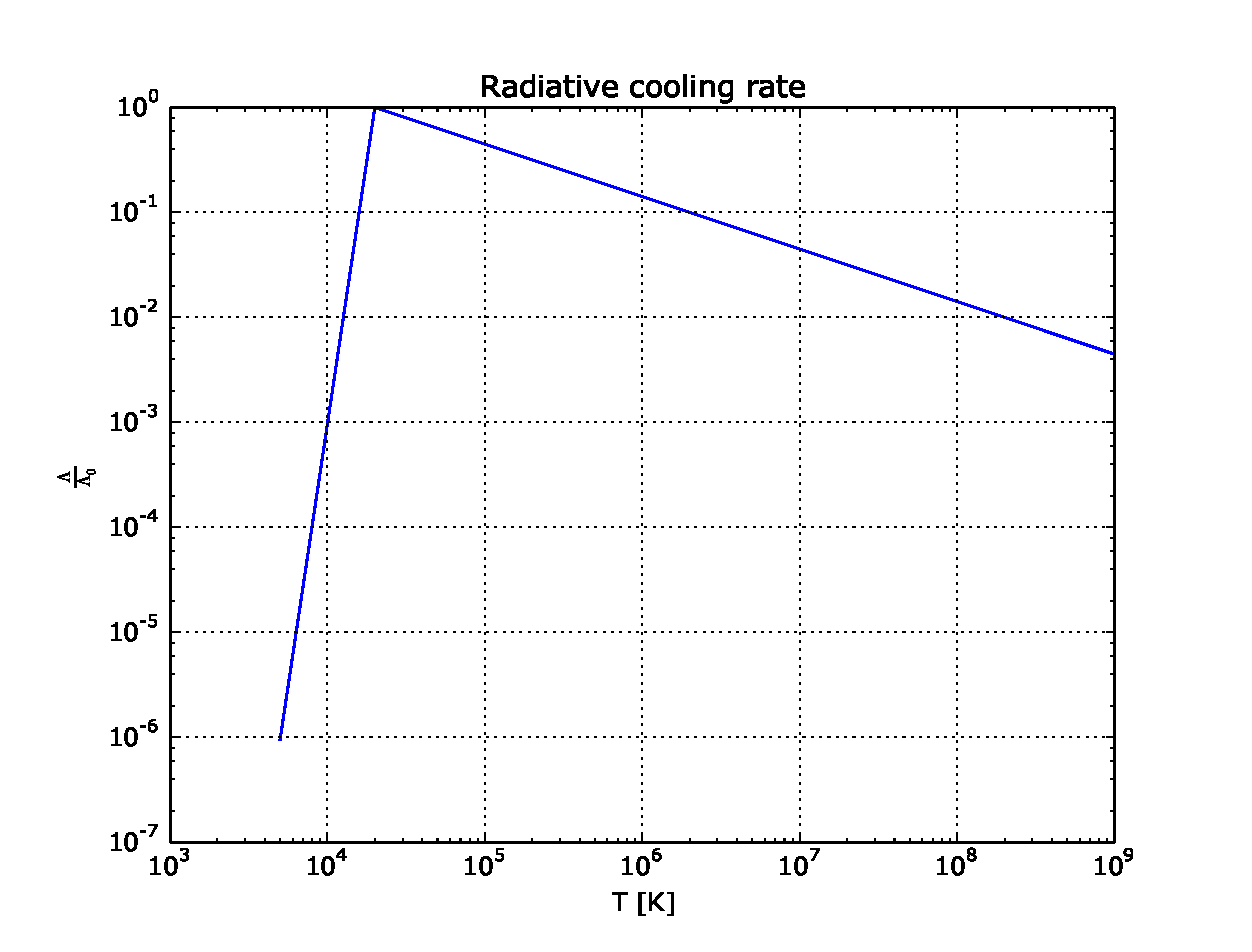
\includegraphics[width=.8\textwidth]{cooling_function.eps}
\end{center}
\caption{Cooling function from the exercise sheet plotted in units of $\Lambda_0$ as a function of the temperature. Please note the strong drop of for $T<20000\,\mathrm{K}$.}\label{fig:cooling function}
\end{figure}

The cooling function from the exercise sheet is plotted in \fref{fig:cooling function}. You can see the peak of the cooling at 20000 K and also the strong drop of for lower temperatures. Expect your simulated plasma to behave accordingly.













\end{document}